%
%  Peter Vermeer
%
\documentclass[12pt,fullpage]{article}
\usepackage{fullpage}
\usepackage{psfrag}                                          % LaTeX graphics tool
\usepackage{pslatex}                                         % avoids the default cmr font
\usepackage{graphicx}                                        % graphics package 
\usepackage{epsfig}                                          % figures
\usepackage{hyperref}
\usepackage{color}

\begin{document}

\noindent
{\bf Standard triangular distribution} (from \color{blue}\url{http://www.math.wm.edu/~leemis/chart/UDR/UDR.html}\color{black})

\noindent
The shorthand $X \sim {\rm triangular}(-1,\, 0,\, 1)$ is used to indicate that the
random variable $X$ has the standard triangular distribution.
A standard triangular random variable $X$ has the probability density function 
$$
f(x) = \left\{ \begin{array}{ll} 
       x +1 & \qquad -1 < x < 0 \\ [0.1in]
       1 - x & \qquad 0 \le x < 1.
       \end{array} \right. 
$$
The probability density function is illustrated below.
{\begin{figure}[h!]
\begin{center}
\psfrag{labx}{$x$}
\psfrag{labf}{$f(x)$}
\psfrag{laba}{$-1$}
\psfrag{labm}{$0$}
\psfrag{labb}{$1$}
\includegraphics[width=3.2in]{StandardtriangularPlot.ps}
\end{center}
\end{figure}}

\noindent
The cumulative distribution function on
the support of $X$ is
$$
F(x) = \left\{ \begin{array}{ll} 
       \frac{1} {2} x ^ {\kern 0.08 em 2} + x + \frac{1} {2} & \qquad -1 < x < 0 \\ [0.1in]
        - \frac{1} {2} x ^ {\kern 0.08 em 2} + x + \frac{1}{2} & \qquad 0 \le x < 1. \\ 
       \end{array} \right. 
$$
The survivor function is
$$
S(x) = \left\{ \begin{array}{ll} 
       -\frac{1} {2} x ^ {\kern 0.08 em 2} - x + \frac{1} {2}& \qquad -1 < x < 0 \\ [0.1in]
       \frac{1} {2} x ^ {\kern 0.08 em 2} - x + \frac{1} {2} & \qquad 0 \le x < 1. 
       \end{array} \right. 
$$
The hazard function is
$$
h(x) = \left\{ \begin{array}{ll} 
      \frac{2 (x + 1)}{-x ^ {\kern 0.08 em 2} - 2x + 1}& \qquad -1 < x < 0 \\ [0.1in]
       \frac{2}{1-x} & \qquad 0 \le x < 1.
       \end{array} \right. 
$$
The cumulative hazard function is
$$
H(x) =  \left\{ \begin{array}{ll} 
      -\ln \left( -\frac{1} {2} x ^ {\kern 0.08 em 2} - x + \frac{1} {2} \right)& \qquad -1 < x < 0 \\ [0.1in]
        -\ln \left(\frac{1} {2} x ^ {\kern 0.08 em 2} - x + \frac{1} {2} \right)& \qquad 0 \le x < 1. 
       \end{array} \right. 
$$
The inverse distribution function of $X$ is
$$
F^{-1}(u) = \left\{ \begin{array}{ll} 
       -1 + \sqrt {2 \kern 0.08 em u} & \qquad 0 < u < \frac{1}{2} \\ [0.1in]
       1 - \sqrt {2 - 2 \, u} & \qquad \frac{1}{2} \le u < 1 .
       \end{array} \right. 
$$
The median of $X$ is 0.
The mode of $X$ is 0.
The moment generating function of $X$ is
$$
M(t) = E\left[ e ^ {\kern 0.08 em tX} \right] = \left\{ \begin{array}{ll}
       1 & \qquad t = 0 \\
       {\frac {{ e ^ {-t}} - 2 + { e ^ {\kern 0.08 em t}}}{{t} ^ {2}}} & \qquad t \ne 0.
       \end{array} \right.
$$
The population mean, variance, skewness, and kurtosis of $X$ are
$$
E[X] = 0 \qquad \qquad 
V[X] = \frac{1} {6} \qquad \qquad 
E\left[ \left( \frac{X - \mu} {\sigma} \right) ^ {\kern -0.08 em 3} \right] = 0 \qquad \qquad 
E\left[ \left( \frac{X - \mu} {\sigma} \right) ^ {\kern -0.08 em 4} \right] = \frac{12} {5}.
$$
An alternate definition of the standard triangular distribution exists. The alternate definition has a minimum of 0, a maximum of 1, and a parameter $m$, representing the mode.

\vspace{0.1in}

\noindent
{\bf APPL verification:}
The APPL statements
\begin{verbatim}
X := TriangularRV(-1,0,1);
CDF(X);
SF(X);
HF(X);
Mean(X);
Variance(X);
Skewness(X);
Kurtosis(X);
MGF(X);
\end{verbatim}
verify the cumulative distribution function, survivor function, hazard function, population mean, variance, skewness, kurtosis, and moment generating function.

\end{document}
